Ein Betrunkener versucht eine Treppe emporzusteigen -- dabei hat er so seine
Probleme, die folgendermassen beschrieben werden können. Dabei sei $p$ eine
reelle Zahl mit $0<p<1$, die als Wahrscheinlichkeit gedeutet wird\footnote{ $p$
steht nicht für ``Promille''! Je grösser $p$ ist, desto ``erfolgreicher'' ist
der Betrunkene.}

\begin{itemize}
 \item Die Treppe besteht aus den $k$ Zuständen (``Stufen'') $S_1 ,S_2, \ldots
	 S_k$. Der Betrunkene startet auf Stufe $S_1$.
 \item Mit jedem Schritt versucht er eine Stufe höher zu kommen, aber folgendes
	 passiert:
       	\begin{itemize}
	\item Wenn sich der Betrunkene auf Stufe $S_j$ mit $j<k$ befindet,
		schafft er es mit Wahrscheinlichkeit $p$ auf die Stufe
		$S_{j+1}$, aber mit Wahrscheinlichkeit $q=1-p$ fällt er auf die
		Stufe $S_1$ zurück.
	\item Wenn sich der Betrunkene auf Stufe $S_k$  befindet, fällt er mit
		Wahrscheinlichkeit $p+q=1$ ganz auf die Anfangsstufe $S_1$
		zurück.
	\end{itemize}
\end{itemize}
\begin{figure}[htbp] %  figure placement: here, top, bottom, or page
   \centering
   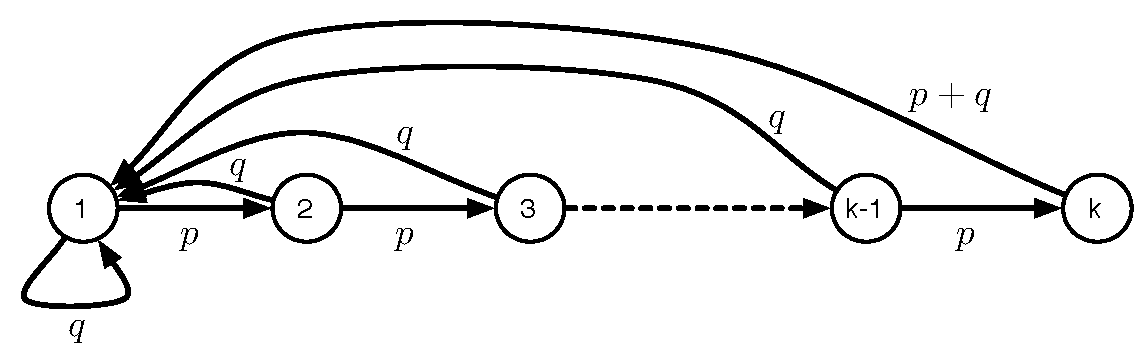
\includegraphics[width=4in]{graphics/devilsgraph.pdf} 
   %\caption{example caption}
   %\label{fig:example}
\end{figure}
Mit $T_k$ soll dieser ``Treppengraph'' bezeichnet werden''. Er hat also Knoten
(Zustände) $\{S_1,S_2,\ldots,S_k\}$ und die Kanten (Transitionen) wie
eingezeichnet.

Sie können diese grafische Darstellung 
\begin{itemize}
\item
entweder als einen endlichen Automaten (mit Startzustand $S_1$) interpretieren,
indem sie $p$ und $q$ als Symbole eines Eingabealphabets betrachten, oder
\item
als Markov-Kette betrachten, bei der die Transitionen zwischen den Zuständen
mit den Wahrscheinlichkeiten $p$ bzw. $q$ geschehen (und keine anderen als die
eingezeichneten vorkommen).
\end{itemize}

Betrachten sie zunächst die Automateninterpretation. Es bezeichne
$Ak_{i,j}^{(n)}$ die Anzahl der Pfade der Länge $n$ von $S_i$ nach $S_j$ in
$T_k$

\begin{flushenum}
\item Geben Sie explizit die Matrizen $Ak = \left[ Ak_{i,j}^{(1)} \right]$ für
	$k=2,3,4$ an und berechnen Sie deren charakteristisches Polynom.
	Welches sind die Eigenwerte?
\item Wie sehen die Matrizen $Ak$ allgemein aus, die das Geschehen in einem
	Schritt auf dieser ``Teufelsleiter'' beschreiben?\\ Zeigen Sie (z.B.
	per Induktion), dass
	\[
	\chi_{Ak}(z) = (z-2) \cdot \frac{z^k-1}{z-1}
	\]
	das charakteristische Polynom der Matrix $Ak$ ist.  Wo liegen die
	Eigenwerte der Matrix $Ak$ in der komplexen Ebene?  Machen Sie sich ein
	Bild davon!\footnote{ Bedenken Sie folgendes: das Polynom $X^k=1$ hat
	in $\mathbb{C}$ die $k$ Nullstellen $e^{2 \pi i (\ell/k)}$ für $0 \leq
	\ell < k$, genannt die (komplexen) $k$-ten Einheitswurzeln, die uns im
	Zusammenhang mit der Diskreten Fouriertransformation noch beschäftigen
	werden. Bezeichnet man mit $\omega_k$ die komplexe Zahl $e^{2 \pi i
	/k}= \cos (2 \pi/k) + i \cdot \sin(2 \pi/k)$, so sind die Nullstellen
	von $X^k=1$ gerade die Zahlen $\omega_k^\ell$ für $0 \leq \ell < k$,
	das sind die Teilungspunkte, wenn man den komplexen Einheitskreis der
	Länge $2 \pi$ in $k$ gleichlange Teile teilt, wobei $\omega_k^0=1$ ein
	Teilungspunkt ist.}
\item Betrachten Sie nun die Folgen
	\[
	\left(Ak_{1,j}^{(n)}\right)_{n \geq 0}~~\text{der Anzahlen der Pfade 
	der Länge $n$ von $S_1$ nach $S_j$ in $T_k$}
	\]
	Diese Folgen sind $C$-rekursiv und haben $\chi_{Ak}(z)$ als
	charakteristisches Polynom. \\
	Wie verhalten sich demnach die Folgen $\left(Ak_{1,j}^{(n)}\right)_{n \geq 0}$ asymptotisch 
	($n \rightarrow \infty$)? Ihre Antwort sollte die Form
	\[
	Ak_{1,j}^{(n)} \sim  \alpha_j \cdot \lambda^n
	\]
	haben. Dabei fragt sich
	\begin{itemize}
	\item Was ist $\lambda$ ? 
	\item Was ist $\alpha_j$ ?
	\end{itemize}
	Die Antwort auf die erste Frage ist einfach. \\
	Für die Antwort auf die zweite Frage bedenken Sie, dass sich aus der
	Problembeschreibung unmittelbar
	\[
	Ak_{1,j}^{(n)} = Ak_{1,j-1}^{(n-1)} ~~~(1<j\leq k)
	\]
	ergibt. Benutzen Sie das asymptotische Verhalten beider Seiten, um $2
	\alpha_j= \alpha_{j-1}$ zu folgern.  Jetzt benötigen Sie nur noch
	\begin{equation*}
		\tag{$*$} \alpha_1+\alpha_2 + \cdots + \alpha_k=1
	\end{equation*}
	um alles zu klären. Die Beziehung $(*)$ erhalten Sie, indem Sie sich
	klarmachen, was
	\[
	Ak_{1,1}^{(n)} + Ak_{1,2}^{(n)} + \cdots + Ak_{1,k}^{(n)} 
	\]
	ist und ebenfalls das asymptotische Verhalten dieser Summe betrachten.
\end{flushenum}

Im folgenden sollten Sie nun die ``stochastische'' Interpretation verwenden.
Dabei geht es um die Frage, auf welcher Stufe $S_\ell$ man den Betrunkenen nach
längerer Zeit mit welcher Wahrscheinlichkeit antrifft?

\begin{flushenum}
\setcounter{itemcounter}{3}
\item Geben Sie die (stochastischen) Matrizen $Ak(p)$ für $k=2,3,4$ explizit
	an, die diese Markovkette beschreiben und berechnen Sie deren
	charakteristisches Polynom.  Welches sind die Eigenwerte?
\item Wie sehen die Matrizen $Ak(p)$ allgemein aus, die das Geschehen in einem
	Schritt auf dieser ``Teufelsleiter''  beschreiben?\\ Zeigen Sie (z.B.
	per Induktion), dass
	\[
	\chi_{Ak(p)}(z) = (z-1) \cdot \frac{z^k-p^k}{z-p}
	\]
	das charakteristische Polynom der Matrix $Ak(p)$ ist.  Wo liegen die
	Eigenwerte der Matrix $Ak(p)$ in der komplexen Ebene?  Machen Sie sich
	ein Bild davon!

\item Es bezeichne nun $\mathtt{P}_\ell^{(n)}$ die Wahrscheinlichkeit, dass der
	Betrunkene nach $n$ Schritten auf der Stufe $S_\ell$ anzutreffen ist.
	Teil 5 der Aufgabe besagt insbesondere, dass $\lambda=1$ ein dominanter
	Eigenwert der Matrix $Ak(p)$ ist.
	Daher gibt es eine eindeutig bestimmte stationäre
	Wahrscheinlichkeitsverteilung $\boldsymbol{\pi}=(\pi_j)_{1 \leq j \leq
	k}$ auf der Menge $\{S_j\,;\, 1 \leq j \leq k\}$  der Zustände und es
	gilt
	\[
	\lim_{n \rightarrow \infty} \mathtt{P}_j^{(n)} = \pi_j ~~~(1 \leq j \leq k).
	\]
	Bestimmen Sie $(\pi_j)_{1 \leq j \leq k}$, indem sie die Beziehung
	\[
	\mathtt{P}_j^{(n)} = \mathtt{P}_{j-1}^{(n-1)} \cdot p~~~(1<j\leq k)
	\]
	und das asymptotische Verhalten verwenden --- ganz analog wie in Teil 3
	dieser Aufgabe.
\end{flushenum}

Hinweis: Das Ganze hat etwas mit einer endlichen geometrischen Reihe zu tun.
Schauen Sie in Kapitel 1 nach, falls Sie vergessen haben, was es damit auf sich
hat.
